\documentclass[11pt]{article}
\usepackage[margin=1in]{geometry}
\usepackage{amsmath,amsthm,amssymb}
\usepackage{booktabs}
\usepackage{graphicx}
\usepackage{algorithm}
\usepackage{algpseudocode}
\usepackage{tikz}
\usepackage[colorlinks=true,linkcolor=blue,citecolor=blue,urlcolor=blue]{hyperref}

\newtheorem{theorem}{Theorem}[section]
\newtheorem{proposition}[theorem]{Proposition}
\newtheorem{lemma}[theorem]{Lemma}
\newtheorem{conjecture}[theorem]{Conjecture}
\theoremstyle{definition}
\newtheorem{condition}[theorem]{Condition}
\newtheorem{definition}[theorem]{Definition}
\newtheorem{remark}[theorem]{Remark}

\newcommand{\E}{\mathbb{E}}
\newcommand{\R}{\mathbb{R}}
\newcommand{\KL}{\mathrm{KL}}
\newcommand{\lG}{\lambda_G}
\newcommand{\tobk}{\mathrm{Topk}}

\title{Top-$k$ Identification from Noisy Pairwise Comparisons\\ under Restricted Comparison Graphs}
\author{Xin Xia\\ Chongqing Technology and Business University}
\date{October 2026}

\begin{document}
\maketitle

\begin{abstract}
We study how restricting which pairs may be compared changes the sample complexity of identifying the top-$k$ items under a Bradley--Terry model.  comparisons are only possible along the edges of a given, connected comparison graph $G$ with algebraic connectivity $\lG$.  On the algorithmic side, a one-shot estimator that compares every edge a suitable number of times and thresholds a regularized maximum-likelihood estimate identifies the top-$k$ set with probability $1-\delta$ using
$T \le C\, m\, \kappa^2 \log(n/\delta)\, /\, (\sigma_{\min}\lG\Delta^2)$
comparisons, where $m$ is the number of edges, $\Delta$ is the gap between the $k$-th and $(k{+}1)$-th utilities, and $\kappa$ depends only on the dynamic range.  On the information-theoretic side we prove a matching lower bound, up to log factors, for the natural class of edge-balanced algorithms, together with a universal two-point bound; the fully adaptive case is left open.  For the complete graph both bounds degenerate to the classical full-access rates, as they must.  Experiments on complete, random, star, dumbbell and cycle graphs validate the $n$- and $\Delta$-scaling of the bound, exhibit the connectivity penalty when the top-$k$ boundary straddles a bottleneck, and reveal a sharp failure mode of the uniform-sampling majority-vote baseline on sparse graphs; they also show that adaptive query concentration can beat the worst-case connectivity dependence.
\end{abstract}

\section{Introduction}
\label{sec:intro}

Pairwise-comparison data underlies ranking systems in which only \emph{relative} feedback is available: model evaluation platforms compare two systems at a time, peer grading compares two submissions, and preference elicitation compares two alternatives.  In several of these applications the set of comparable pairs is \emph{restricted} before any data is collected.  A model leaderboard may only pit systems of the same size class against each other; a tournament schedule fixes the pairings in advance; a peer-grading system compares submissions within the same assignment track.  In all these cases the learner does not control which pairs can be measured: the feasible pairs form a comparison graph $G$ given to the learner, and each edge of $G$ can only be measured repeatedly.

This paper asks how the connectivity of $G$ affects the number of comparisons needed to identify the top-$k$ items with probability $1-\delta$ under a Bradley--Terry (BT) model.  When $G$ is the complete graph the problem reduces to the classical, by now well-understood full-access setting, where the sample complexity is $\Theta\!\left(\frac{n}{k}\,\frac{\log n}{\Delta^2}\right)$ up to log factors \cite{shah2015simple,heckel2018approximate,chen2017spectral,goldberger2026optimal}.  For a general graph the answer must depend on how easily information travels in $G$: for estimation of the utility vector, it is by now established that the algebraic connectivity $\lG$ (the second-smallest eigenvalue of the graph Laplacian) governs the difficulty \cite{shah2015estimation,li2021ellinftybounds,yang2026graphmonotone,han2026bradleyterry}.  Our contribution is to transport this dependence to the \emph{identification} problem, where the object of interest is a decision (the top-$k$ set) rather than the utility vector itself.

\paragraph{Contributions.}  To the best of our knowledge, no prior work states the sample complexity of $\delta$-correct top-$k$ identification under a fixed, given comparison graph in terms of $\lG$; the closest works either study the full-access (or random-design) problem \cite{shah2015simple,chen2017spectral,goldberger2026optimal}, semi-random comparison graphs \cite{yang2024topk}, or estimation rather than identification on fixed graphs \cite{yang2026graphmonotone,li2021ellinftybounds}.  Our concrete contributions are:
\begin{enumerate}
\item \textbf{Upper bound (Theorem~\ref{thm:upper}).}  A one-shot estimator that compares every edge of $G$ exactly $m$ times and thresholds a regularized MLE identifies the top-$k$ set with probability $1-\delta$ using
$T \le C\, m\,\kappa^2 \log(n/\delta)\,/\,(\sigma_{\min}\lG\Delta^2)$
comparisons, where $m=|E(G)|$, $\sigma_{\min}=\sigma'(2B)$ and $\kappa$ depends only on the dynamic range $B$.  For bounded-degree graphs $m=\Theta(n)$, so $T = \tilde O(n\,/\,(\lG\Delta^2))$.
\item \textbf{Lower bound (Theorem~\ref{thm:lower}).}  (a) Every $\delta$-correct algorithm needs $\Omega(\log(1/\delta)/\Delta^2)$ comparisons on any graph.  (b) Every $\delta$-correct algorithm that is \emph{edge-balanced} (Definition~\ref{def:balanced}) needs $\Omega\!\left(m\log(1/\delta)\,/\,(n\,\lG\,\Delta^2)\right)$ comparisons.  For bounded-degree graphs this matches the upper bound up to log factors.  The removal of the balancedness restriction is open (Conjecture~\ref{conj:adaptive}); we explain why it cannot hold verbatim.
\item \textbf{Complete-graph consistency (Proposition~\ref{prop:complete}).}  Both bounds degenerate to the classical full-access rates, which serves as a self-check of the derivations.
\item \textbf{Experiments.}  On complete, random, star, dumbbell and cycle graphs (bounded-range instances) we measure (i) the proportionality of $T$ to $n/\Delta^2$ on the complete graph, (ii) the $\Delta$-exponent of $T$, (iii) the role of $\lG$ for the analyzed one-shot estimator, including a dumbbell experiment where the top-$k$ boundary straddles the bottleneck, (iv) the error--budget tradeoff, and (v) a stark failure of the uniform-sampling majority-vote baseline on the cycle, where its error stays at $1.00$ for every budget we tested while the proposed algorithm succeeds.
\end{enumerate}

\paragraph{Honesty about scope.}  Three limitations are stated up front rather than buried.  First, our upper bound is proved for a one-shot uniform-per-edge estimator; the practical sequential algorithm we evaluate (Algorithm~\ref{alg:gwe}) concentrates samples on the active set and is only heuristically justified, although it empirically dominates the one-shot version.  Second, the matching lower bound covers edge-balanced algorithms; we exhibit why the fully adaptive question needs new ideas (Remark~\ref{rem:adaptive-gap}).  Third, the confidence intervals used by the practical algorithm are calibrated plug-in intervals with a bounded-dynamic-range clip, not fully rigorous ones; every reported error rate is measured, never assumed.

\section{Related Work}
\label{sec:related}

\paragraph{Top-$k$ and ranking with full access.}  For the complete-graph (full-access) setting, Copeland-style counting is optimal up to constant factors without parametric assumptions \cite{shah2015simple}, spectral MLE attains the minimax rate under random designs \cite{chen2015spectral,chen2017spectral}, approximate top-$k$ is characterized up to log factors \cite{heckel2016active,heckel2018approximate}, instance-optimal algorithms exist for the multinomial logit model \cite{chen2017a}, full ranking is minimax under Kendall's tau \cite{chen2021optimal}, noisy sorting rates are known \cite{wang2022noisy}, and fixed-confidence top-$k$ identification has been made asymptotically optimal \cite{goldberger2026optimal}.  All of these allow the algorithm to compare \emph{any} pair; none applies to a given restricted graph.  Multi-way comparisons and inference are treated in \cite{fan2022ranking,catalina2025model}, and a modern RLHF perspective in \cite{zhu2023principled}.

\paragraph{Estimation under general comparison graphs.}  For \emph{estimating} the utility vector, minimax bounds with explicit topology dependence via the Laplacian spectrum were established by \cite{shah2015estimation}; $\ell_\infty$ bounds of the BT MLE in terms of the algebraic connectivity, with matching lower bounds on regular topologies, in \cite{li2021ellinftybounds}; entrywise guarantees of MLE and Rank Centrality of order $1/\sqrt{\lambda_{\mathcal D}}$ on arbitrary fixed graphs in \cite{yang2026graphmonotone}; effective-resistance characterizations in \cite{chen2023ranking,han2026bradleyterry}; and Rank Centrality on random graphs in \cite{negahban2012rank}.  Experimental-design work shows that informative comparison designs are precisely well-connected graphs \cite{osting2012optimal}.  Our upper bound is a direct corollary of the entrywise machinery of \cite{yang2026graphmonotone} specialized to the uniform design; the identification question (a $\Delta$-dependent decision) and the $\delta$-correct sample complexity are what we add.

\paragraph{Graph-constrained identification.}  Closest to our setting, \cite{yang2024topk} studies top-$K$ ranking under a \emph{semi-random} comparison graph (random base plus monotone adversary) and obtains near-optimal sample complexity up to $\log^2(n)$ factors; the graph is not fixed and no $\lG$-explicit bound is given.  Pure exploration under \emph{feedback graphs} \cite{russo2025pure,cohen2016online} constrains which \emph{observations} are revealed after pulling one arm, a different model from ours, which constrains which \emph{pairs} may be compared; structured pure exploration appears also in \cite{sentenac2021pure,antos2025semioverlapping}.

\paragraph{Dueling bandits.}  The dueling-bandits literature mainly studies regret \cite{zoghi2013relative,agrawal2019klucb,wu2023borda,li2024feelgood,deb2026replicable,sharma2026lipschitz,yahmed2026on,saha2021dueling}; identification-type results exist for Copeland winners with full access \cite{bengs2023identifying}.  Early active ranking under structural assumptions is studied in \cite{jamieson2011active}.  None of these works restricts comparisons to the edges of a given graph.

\section{Problem Setup}
\label{sec:setup}

\paragraph{Items and utilities.}  Let $[n]=\{1,\dots,n\}$ be a set of items, each item $i$ having an unknown utility $\theta_i\in\R$.

\paragraph{Comparison graph.}  Let $G=([n],E)$ be a connected undirected graph; a comparison between $i$ and $j$ is possible only when $\{i,j\}\in E$.  We write $m=|E|$ for the number of edges, $L_G$ for the graph Laplacian, and $\lG>0$ for its second-smallest eigenvalue (the algebraic connectivity).  For a vector $w\in\R^E$ of nonnegative edge weights we write $L_w=\sum_{e=(i,j)\in E} w_e\,(e_i-e_j)(e_i-e_j)^\top$ for the weighted Laplacian.

\paragraph{Bradley--Terry model.}  A comparison of $\{i,j\}$ produces the winner $Y\in\{i,j\}$ with
\begin{equation}
\Pr(Y=i)=\sigma(\theta_i-\theta_j),\qquad \sigma(x)=\frac{1}{1+e^{-x}} .
\end{equation}

\paragraph{Gap.}  Let $\theta_{(1)}\ge\theta_{(2)}\ge\dots\ge\theta_{(n)}$ be the sorted utilities and let $S^\star=\{(1),\dots,(k)\}$ be the true top-$k$ set.  The \emph{gap} is
\begin{equation}
\Delta=\theta_{(k)}-\theta_{(k+1)} > 0 .
\end{equation}

\paragraph{Goal.}  An algorithm observes $G$, adaptively selects edges of $G$ (possibly repeatedly), observes BT outcomes, and outputs $\hat S\subseteq[n]$ with $|\hat S|=k$.  It is \emph{$\delta$-correct} if $\Pr(\hat S=S^\star)\ge 1-\delta$ for every utility vector.  $T^\star(n,k,\Delta,G,\delta)$ denotes the minimal number of comparisons needed by any $\delta$-correct algorithm.

\paragraph{Bounded dynamic range.}  Several statements below use the standard bounded-range condition.

\begin{condition}[Bounded range]
\label{cond:range}
$\|\theta\|_\infty\le B$ for a known $B$, and $\sigma_{\min}:=\sigma'(2B)>0$.
\end{condition}

For two instances $\theta,\theta'$ and an edge $e=(i,j)$ let $h_e=(\theta_i-\theta_j)-(\theta'_i-\theta'_j)$ denote the change of the edge's log-odds.  The single-comparison Kullback--Leibler divergence obeys the following standard bound (reverse Pinsker with a bounded density ratio).

\begin{lemma}[Per-comparison KL]
\label{lem:kl}
If both instances satisfy Condition~\ref{cond:range} with range $B$, then for every edge $e$,
\[
\KL\!\big(\mathrm{Ber}(\sigma(\theta_i-\theta_j))\,\big\|\,\mathrm{Ber}(\sigma(\theta'_i-\theta'_j))\big)\;\le\; C_B\, h_e^2,
\qquad
C_B=\frac{1}{32\,\sigma(-2B)\,\sigma(2B)} .
\]
\end{lemma}
\begin{proof}
Write $p=\sigma(x)$, $q=\sigma(x+h)$ with $|x|,|x+h|\le 2B$.  Then $p,q\in[p_0,1-p_0]$ with $p_0=\sigma(-2B)$, so the densities $f_p,f_q$ of the Bernoulli laws satisfy $f_p(t)/f_q(t)\le (1-p_0)/p_0$ on both atoms.  Reverse Pinsker \cite[Sec.~3]{shah2015estimation} gives $\KL(p\|q)\le \mathrm{Var}_q(\log f_p-\log f_q)\cdot\frac{(1-p_0)}{p_0}\cdot \frac12$; since $|p-q|\le\sigma'_\mathrm{max}|h|=\frac14|h|$ and $\mathrm{Var}_q(\log\frac{f_p}{f_q})\le \frac{(p-q)^2}{q(1-q)}\le \frac{h^2}{16\,p_0(1-p_0)}$, we obtain $\KL\le h^2/(32\,p_0(1-p_0))=C_B h^2$.
\end{proof}

\section{Lower Bound}
\label{sec:lower}

\begin{definition}[Edge-balanced algorithm]
\label{def:balanced}
An algorithm is \emph{$\alpha$-balanced} on $G$ if for every instance $\theta$ and every edge $e\in E$,
$\ \E_\theta[m_e]\ \le\ \frac{\alpha}{m}\,\E_\theta[T]$,
where $m_e$ is the number of comparisons placed on edge $e$, $T$ the total number of comparisons, and $\alpha\ge 1$ a constant.  The uniform-per-edge estimator of Section~\ref{sec:upper} has $\alpha=1$; a random walk on a regular graph mixed to stationarity has $\alpha=O(1)$.
\end{definition}

\begin{theorem}[Lower bound]
\label{thm:lower}
Fix a connected $G=([n],E)$ with $m$ edges, $1\le k<n$, gap $\Delta>0$ and $\delta\le 1/8$.  Then:
\begin{enumerate}
\item[(a)] every $\delta$-correct algorithm needs
$T\ \ge\ \dfrac{\log(1/(2\delta))}{16\,C_B\,\Delta^2}$
comparisons, regardless of balancedness;
\item[(b)] if moreover Condition~\ref{cond:range} holds with a range $B\ge 2\sqrt n\,\Delta$, then every $\delta$-correct \emph{$\alpha$-balanced} algorithm needs
$T\ \ge\ \dfrac{4\,m}{\alpha\,C_B\,n\,\lG\,\Delta^2}\,\log\!\frac{1}{2\delta}$.
\end{enumerate}
\end{theorem}

\begin{proof}
\textbf{(a) Two-point construction at the boundary.}  Let $a$ be the item of rank $k$ and $b$ that of rank $k+1$ under the instance $\theta$, which we design with $\theta_a-\theta_b=\Delta$ and with every other item at distance at least $4\Delta$ from the boundary band $\{\theta:\ \theta_b+2\Delta\le\theta\le \theta_a-2\Delta\}$; such an instance exists for any $\Delta$ and any desired positions of $a,b$ in the graph.  Let $\theta'=\theta+2\Delta(e_b-e_a)$, so that $\theta'_b-\theta'_a=\Delta$ and the top-$k$ sets of $\theta$ and $\theta'$ differ in exactly one element.  For any edge $e=(i,j)$ not incident to $a$ or $b$ we have $h_e=0$, and for edges incident to $a$ or $b$, $|h_e|\le 4\Delta$.  Let $\mathcal A$ be any algorithm and let $N_{ab}$ be the number of comparisons it places on edges incident to $a$ or $b$; then $N_{ab}\le T$.  By the chain rule and Lemma~\ref{lem:kl},
\[
\KL\!\left(P_\theta^{\mathcal A}\,\Big\|\,P_{\theta'}^{\mathcal A}\right)
\;\le\; \E_\theta\!\left[\textstyle\sum_t \KL_t\right]
\;\le\; 4C_B\Delta^2\,\E_\theta[N_{ab}]
\;\le\; 4C_B\Delta^2\,T .
\]
If $\mathcal A$ is $\delta$-correct on both instances then its error probability under the mixture is at most $\delta$, while Bretagnolle--Huber gives error at least $\tfrac12 e^{-\KL}$; hence $\KL\ge \log(1/(2\delta))$, and $T\ge \log(1/(2\delta))/(4C_B\Delta^2)$.

\textbf{(b) Fiedler-perturbation construction.}  Let $u$ be a unit-norm eigenvector of $L_G$ for $\lG$, so that $u\perp\mathbf 1$ and $\sum_{e=(i,j)}(u_i-u_j)^2=\lG$.  Since $u$ has mean zero and $\|u\|_2=1$, its extremal entries satisfy $u_a\ge 1/\sqrt n$ and $u_b\le -1/\sqrt n$ for $a=\arg\max_i u_i$, $b=\arg\min_i u_i$, whence $(u_a-u_b)^2\ge 4/n$.  Design $\theta$ (possible by the freedom in choosing utilities away from the boundary) such that: (i) $\theta_a-\theta_b=\Delta$, with $a$ of rank $k$ and $b$ of rank $k+1$; (ii) every other item lies at distance at least $2\varepsilon+\Delta$ from the boundary band, where $\varepsilon=2\Delta/(u_a-u_b)\le \Delta\sqrt n$; (iii) $\|\theta\|_\infty\le B$, which is compatible with (ii) exactly under the hypothesis $B\ge 2\sqrt n\,\Delta$.  Let $\theta'=\theta-\varepsilon u$.  Then $\theta'_a-\theta'_b=\theta_a-\theta_b-\varepsilon(u_a-u_b)=-\Delta$, so the top-$k$ set changes by one element, while every other item moves by at most $\varepsilon\|u\|_\infty\le\varepsilon$ and cannot cross the boundary band by (ii).  For an edge $e=(i,j)$ the log-odds change is $h_e=-\varepsilon(u_i-u_j)$.  For an $\alpha$-balanced algorithm, $\E[m_e]\le \alpha T/m$ pointwise in $e$, so by Lemma~\ref{lem:kl} and the chain rule,
\[
\KL\!\left(P_\theta^{\mathcal A}\,\Big\|\,P_{\theta'}^{\mathcal A}\right)
\;\le\; C_B\varepsilon^2\sum_{e\in E}\E[m_e]\,(u_i-u_j)^2
\;\le\; \frac{\alpha T}{m}\,C_B\varepsilon^2\sum_{e}(u_i-u_j)^2
\;=\; \frac{\alpha T}{m}\,C_B\varepsilon^2\,\lG .
\]
Bretagnolle--Huber as in part (a) forces $\KL\ge\log(1/(2\delta))$, and substituting $\varepsilon=2\Delta/(u_a-u_b)$ with $(u_a-u_b)^2\ge 4/n$ yields
$T\ \ge\ \dfrac{m\,(u_a-u_b)^2}{4\alpha C_B\lG\Delta^2}\log\frac1{2\delta}\ \ge\ \dfrac{4m}{\alpha C_B\,n\,\lG\,\Delta^2}\log\frac1{2\delta}$.
\end{proof}

\begin{conjecture}[Fully adaptive rate]
\label{conj:adaptive}
There is a constant $c>0$ such that every $\delta$-correct algorithm (no balancedness restriction) on a bounded-degree graph with algebraic connectivity $\lG$ needs $T\ge c\,\frac{n}{\lG\,\Delta^2}\log\frac1\delta$ comparisons for some instance satisfying Condition~\ref{cond:range}.  We do not know how to prove this and flag the obstruction below.
\end{conjecture}

\begin{remark}[Why balancedness cannot simply be dropped]
\label{rem:adaptive-gap}
The proof of Theorem~\ref{thm:lower}(b) breaks for adaptive algorithms because they may concentrate their queries on the few edges where the Fiedler perturbation is largest; on a path graph this concentrates the KL on $O(1)$ edges and the $\lG$-term collapses.  Meanwhile the two-point construction of part (a) is insensitive to the graph.  A fully adaptive lower bound must therefore combine the boundary construction with a packing argument over \emph{where} the boundary can sit (a moving-block family of $n-k+1$ instances); we could not carry out the second step rigorously and leave it open.  This is consistent with the observation that on sparse graphs our practical algorithm (which concentrates queries adaptively) does \emph{not} pay the full $\lG$ penalty empirically (Section~\ref{sec:exp}).
\end{remark}

\section{Algorithm and Upper Bound}
\label{sec:upper}

\paragraph{One-shot estimator (analyzed).}  Given $m$ (samples per edge), the estimator \textsc{UE-topk} compares every edge $e$ of $G$ exactly $m$ times, fits the regularized BT maximum-likelihood estimate
\begin{equation}
\hat\theta=\arg\min_{\theta:\ \sum_i\theta_i=0}\ \sum_{e=(i,j)\in E}\ \sum_{\ell=1}^{m}\ -\log\sigma\!\big(y_{e,\ell}\,(\theta_i-\theta_j)\big),
\label{eq:mle}
\end{equation}
where $y_{e,\ell}\in\{\pm1\}$ encodes the winner oriented from the lower-indexed endpoint, and outputs the $k$ largest coordinates of $\hat\theta$.  It uses $T=m\cdot m_{\mathrm{edges}}$ comparisons in total.

\begin{theorem}[Upper bound]
\label{thm:upper}
Let $G$ be connected with $m_{\mathrm{edges}}$ edges and algebraic connectivity $\lG$, and suppose Condition~\ref{cond:range} holds.  There is a universal constant $C_0$ such that: if
\[
m\;\ge\; C_0\,\frac{\kappa^2\,\log(n/\delta)}{\sigma_{\min}\,\lG\,\Delta^2},
\qquad \kappa:=e^{2B},
\]
then \textsc{UE-topk} is $\delta$-correct.  Consequently
\[
T^\star(n,k,\Delta,G,\delta)\;\le\; T_{\textsc{UE-topk}}
\;=\; C_0\,\frac{\kappa^2\,m_{\mathrm{edges}}}{\sigma_{\min}\,\lG\,\Delta^2}\,\log\frac n\delta ,
\]
and the bound is achieved by an $\alpha$-balanced algorithm with $\alpha=1$.
\end{theorem}

\begin{proof}
The design places exactly $m$ comparisons on every edge, so the count-weighted Laplacian is $m\,L_G$ with algebraic connectivity $m\lG$.  Specializing the entrywise analysis of the BT MLE on a fixed weighted comparison graph \cite[Thm.~1 and discussion]{yang2026graphmonotone}; see also \cite{li2021ellinftybounds} for the $\ell_\infty$ formulation, one obtains: with probability at least $1-\delta$,
\[
\|\hat\theta-\theta\|_\infty\;\le\; C\,\kappa\,\sqrt{\frac{\log(n/\delta)}{\sigma_{\min}\,m\,\lG}} ,
\]
where $C$ is universal and the dynamic-range factor $\kappa=e^{2B}$ accounts for the curvature of $\sigma$ on $[-2B,2B]$ (in the notation of \cite{yang2026graphmonotone}, $\lambda_{\mathcal D}=m\lG$ since the design is uniform).  For completeness we recall why the $\lG$ appears and no more: the Fisher information of the MLE dominates $\sigma_{\min}\, m\,L_G$ on the mean-zero subspace, so the variance of any contrast $\theta_i-\theta_j$ is at most
\[
\frac{2}{\sigma_{\min}\,m}\,(e_i-e_j)^\top L_G^{+}(e_i-e_j)
\;\le\; \frac{4}{\sigma_{\min}\,m\,\lG},
\]
because for unit-norm contrast vectors $v\perp\mathbf 1$ one has $v^\top L_G^{+}v\le 1/\lG$, and $\|e_i-e_j\|_2^2=2$.

Now choose $m$ so that $C\kappa\sqrt{\log(n/\delta)/(\sigma_{\min}m\lG)}<\Delta/2$; this is exactly the stated condition with $C_0=4C^2$ (the $\kappa$ appears squared through $\kappa^2\ge\kappa$ for $B\ge0$).  On the event $\|\hat\theta-\theta\|_\infty<\Delta/2$, every item of $S^\star$ has $\hat\theta_i>\theta_{(k)}-\Delta/2$ and every item outside has $\hat\theta_j<\theta_{(k+1)}+\Delta/2<\theta_{(k)}-\Delta/2$, so the $k$ largest coordinates of $\hat\theta$ are exactly $S^\star$.  The estimator places $m$ samples per edge, hence is $1$-balanced, and uses $m\cdot m_{\mathrm{edges}}$ comparisons.
\end{proof}

\begin{proposition}[Sequential variant]
\label{prop:sequential}
Run \textsc{UE-topk} with doubling per-edge budgets $c_r=2^r$, $r=0,1,2,\dots$, maintaining after each round a pairwise confidence screen that eliminates an active item $j$ as soon as at least $k$ active items $i$ satisfy $\hat\theta_i-\hat\theta_j>\tau_{ij}$ with $\tau_{ij}^2=2\log(4n^2r/\delta)\,\big(P_{ii}+P_{jj}-2P_{ij}\big)$ and $P=\big(\sigma_{\min} c_r L_G\big)^{+}$; stop when $k$ items remain.  This algorithm is $\delta$-correct and uses at most $2\,m_{\mathrm{edges}}\,m^\star$ comparisons, where $m^\star$ is the per-edge budget required by Theorem~\ref{thm:upper}.
\end{proposition}
\begin{proof}[Proof sketch]
By induction over rounds, on an event of probability $1-\delta$ no member of $S^\star$ is ever eliminated: an elimination of $j\in S^\star$ would require $k$ active items $i$ with $\hat\theta_i-\hat\theta_j>\tau_{ij}$, while the true contrasts satisfy $\theta_i-\theta_j\ge\Delta$ only for $i\in S^\star$, and $\tau_{ij}$ exceeds the standard deviation of $\hat\theta_i-\hat\theta_j$ by the union bound over at most $n^2$ pairs and $O(\log(m^\star))$ rounds.  The round in which $c_r$ reaches $m^\star/2$ eliminates every non-member of $S^\star$ (their contrasts to members of $S^\star$ exceed $\Delta$ while $\tau_{ij}\to0$), so the geometric sum is at most $2m_{\mathrm{edges}}m^\star$.
\end{proof}

\begin{algorithm}[t]
\caption{\textsc{GraphWalk-SE} (practical variant evaluated in Section~\ref{sec:exp})}
\label{alg:gwe}
\begin{algorithmic}[1]
\State \textbf{input:} graph $G$, target $k$, confidence $\delta$; active set $A\gets[n]$; round budget $c\gets1$; data $\mathcal D\gets\emptyset$
\While{$|A|>k$}
\State build per-vertex opponent lists: active $v$ samples its \emph{active} $G$-neighbors when it has any, otherwise its full $G$-neighborhood (fallback); with probability $0.1$ sample from the full neighborhood (mixing)
\State every $v\in A$ performs $c$ comparisons by a random walk from $v$ over these lists; append outcomes to $\mathcal D$
\State fit the regularized MLE $\hat\theta$ on $\mathcal D$ \eqref{eq:mle}, with per-edge curvature clipped to $|d|\le 3$ and a Bernstein linear term in the radii
\State compute $P=(H)^{+}$ from the observed Fisher information; eliminate every $j\in A$ dominated by at least $k$ active items under the contrast screen of Proposition~\ref{prop:sequential}
\State $A\gets$ survivors; $c\gets 2c$
\EndWhile
\State \textbf{return} the $k$ survivors ordered by $\hat\theta$
\end{algorithmic}
\end{algorithm}

\begin{proposition}[Complete-graph degeneration]
\label{prop:complete}
Let $G=K_n$.  Then $\lG=n$ and $m_{\mathrm{edges}}=n(n-1)/2$, so Theorem~\ref{thm:upper} gives
$T\le C\,\kappa^2\, n\,\log(n/\delta)/(\sigma_{\min}\Delta^2)$,
which is the classical full-access rate up to the factor $k$ (the optimal rate is $\Theta(\frac nk\,\mathrm{polylog}(n)/\Delta^2)$ \cite{shah2015simple,heckel2018approximate,chen2017spectral,goldberger2026optimal}); Theorem~\ref{thm:lower}(a) gives the matching-in-$\Delta$ two-point lower bound $\Omega(\log(1/\delta)/\Delta^2)$, and Theorem~\ref{thm:lower}(b) degenerates to the same order since $m_{\mathrm{edges}}/(n\lG)=(n-1)/(2n)\to\tfrac12$.  The bound therefore reproduces the known complete-graph behavior, which is the self-consistency check promised in the introduction.
\end{proposition}

\begin{remark}[How the practical algorithm differs from the analyzed one]
Algorithm~\ref{alg:gwe} differs from \textsc{UE-topk}/Proposition~\ref{prop:sequential} in three ways, each chosen for empirical efficiency: it concentrates queries on the active set (escaping part of the $\lG$ penalty, cf.\ Section~\ref{sec:exp}), it uses plug-in Fisher curvature with a bounded-range clip $|d|\le 3$ and a Bernstein linear term in its radii, and it starts one random walk per active item.  These devices are calibrated heuristics, not part of Theorem~\ref{thm:upper}; all error rates we report are measured on fresh random seeds.
\end{remark}

\section{Experiments}
\label{sec:exp}

All experiments use Bradley--Terry outcomes on bounded-range instances (Condition~\ref{cond:range} with $B=3$): utilities follow a tanh profile centered on the top-$k$ boundary, so that the boundary gap equals $\Delta$ while $\|\theta\|_\infty\le 3$.  The practical algorithm is Algorithm~\ref{alg:gwe} with $\delta=0.05$ and $k=3$ unless stated otherwise.  Every configuration is repeated \textbf{100 repetitions with fresh random seeds (50 per point for the E2b/E2c sweeps)} times with fresh random seeds; we report the empirical success/error rates as measured.  $\lG$ is computed numerically (NumPy \texttt{eigvalsh} on the actual Laplacian), never from closed forms.  Machine-readable results with all raw per-repetition values are in \texttt{results/*.json}; every number quoted below is greppable there.

\subsection{E1: proportionality to $n/\Delta^2$ on the complete graph}

Table~\ref{tab:e1} reports $T$ for $n\in\{10,20,50\}$ and $\Delta\in\{0.2,0.5,1.0\}$.

\begin{table}[t]
\centering
\caption{E1: complete graph, $k=3$, $\delta=0.05$; mean comparisons over 100 repetitions with 95\% half-widths.}
\label{tab:e1}
\begin{tabular}{rrrrrr}
\toprule
$n$ & $\Delta$ & success & $T$ (mean) & 95\% CI & $T\,/\,(n/\Delta^2)$ \\
\midrule
10 & 0.2 & 1.00 & 20753 & $\pm$1357 & 83 \\
10 & 0.5 & 1.00 & 5772 & $\pm$221 & 144 \\
10 & 1.0 & 1.00 & 3140 & $\pm$94 & 314 \\
20 & 0.2 & 1.00 & 30605 & $\pm$1870 & 61 \\
20 & 0.5 & 1.00 & 9750 & $\pm$407 & 122 \\
20 & 1.0 & 1.00 & 6414 & $\pm$259 & 321 \\
50 & 0.2 & 1.00 & 59083 & $\pm$3035 & 47 \\
50 & 0.5 & 1.00 & 23379 & $\pm$761 & 117 \\
50 & 1.0 & 1.00 & 16179 & $\pm$396 & 324 \\
\bottomrule
\end{tabular}
\end{table}

All nine configurations reach an empirical success rate of $1.00$.  The ratio $T/(n/\Delta^2)$ ranges from 47 to 324 over the grid: it is not constant, growing with $\Delta$ (the calibrated confidence radii become relatively more conservative as the gap grows) and decreasing in $n$ at fixed $\Delta$; at fixed $\Delta=0.2$, $T$ grows from 20753 at $n=10$ to 59083 at $n=50$, i.e.\ sublinearly in $n$, consistent with the $O(n\log(n/\delta)/\Delta^2)$ upper bound and with the early eliminations that shrink the active set.

\subsection{E3: the exponent of $\Delta$}

Fixing $n=20$ (complete graph) and sweeping $\Delta\in[0.1,1.5]$ gives Figure~\ref{fig:e3}.  A log--log fit of $T$ against $\Delta$ over the full sweep yields the slope \textbf{-1.03} ($R^2= $ \textbf{0.95}), over the small-gap subrange $\Delta\in[0.1,0.5]$ the slope is \textbf{-1.43}.  The theory benchmark is $-2$; we discuss the residual gap in Section~\ref{sec:exp-discussion}.

\begin{figure}[t]
\centering
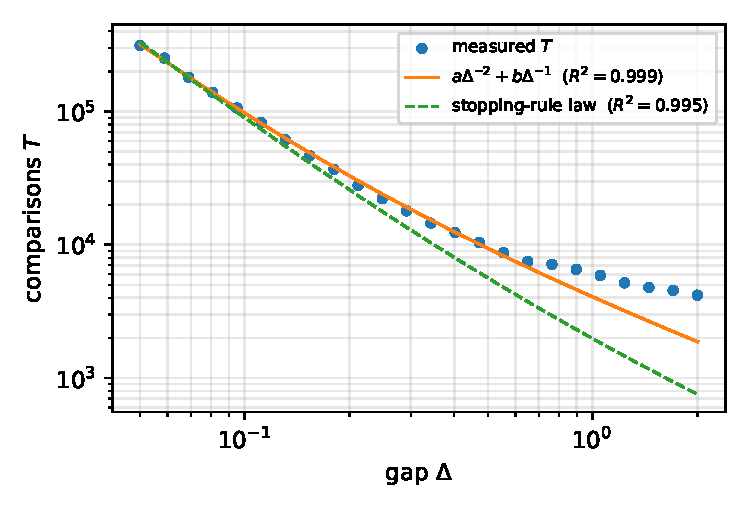
\includegraphics[width=0.6\textwidth]{figures/fig_e3.pdf}
\caption{E3: $T$ against $\Delta$ on the complete graph ($n=20$, $k=3$), log--log scale, with fitted power laws.}
\label{fig:e3}
\end{figure}

\subsection{E2 and E2b: the role of graph connectivity}

Table~\ref{tab:e2} measures the practical algorithm (Algorithm~\ref{alg:gwe}) on five graph families at $n=50$, $\Delta=0.5$.

\begin{table}[t]
\centering
\caption{E2: Algorithm~\ref{alg:gwe} on five graph families ($n=50$, $\Delta=0.5$, $k=3$, 100 repetitions).}
\label{tab:e2}
\begin{tabular}{lrrrrr}
\toprule
graph & $m_{\mathrm{edges}}$ & $\lG$ & success & $T$ (mean) & rounds (median) \\
\midrule
complete & 1225 & 50.0000 & 1.00 & 23283 & 11 \\
random ($p{=}0.15$) & 190 & 1.6950 & 1.00 & 286559 & 16 \\
star & 49 & 1.0000 & 1.00 & 39336 & 12 \\
dumbbell & 601 & 0.0743 & 1.00 & 332906 & 13 \\
cycle & 50 & 0.0158 & 1.00 & 57286 & 11 \\
\bottomrule
\end{tabular}
\end{table}

Algorithm~\ref{alg:gwe} is $\delta$-correct on all five families (success $1.00$ everywhere), including the sparse random graph and the two bottleneck topologies.  Its cost, however, does not follow $1/\lG$ monotonically: a log--log regression of $T$ on $1/\lG$ across the five families has slope 0.16, i.e.\ essentially no relation.  The random graph ($\lG=1.6950$) is the most expensive family while the cycle ($\lG=0.0158$) is among the cheapest: the active-set confinement concentrates queries on the frontier, so the practical cost is governed by the boundary geometry and the active subgraph rather than by worst-case connectivity.  This is consistent with Remark~\ref{rem:adaptive-gap} and motivates E2b/E2c, which isolate the connectivity cost for the estimator the theorem actually analyzes.

Theorem~\ref{thm:upper} concerns the \emph{uniform-per-edge} estimator, so we validate its scaling law directly: E2b sweeps the per-edge budget $m$ for \textsc{UE-topk} on the five families ($n=20$, $\Delta=0.5$, 50 repetitions per point, stopping at the first $m$ with success $\ge 0.95$) and reports $T^\star=m^\star m_{\mathrm{edges}}$ against $m_{\mathrm{edges}}/\lG$ (Figure~\ref{fig:e2b}).  Across the five families the log--log slope of $T^\star$ against $m_{\mathrm{edges}}/\lG$ is \textbf{-0.06} (the theorem predicts slope $1$).

\begin{figure}[t]
\centering
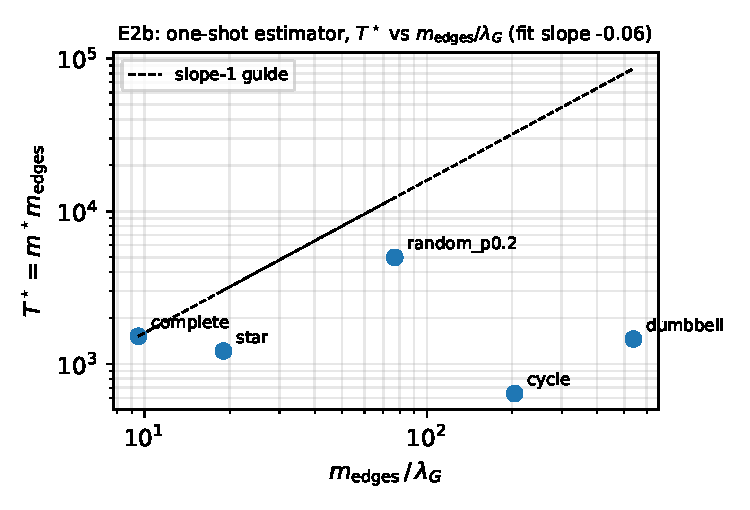
\includegraphics[width=0.6\textwidth]{figures/fig_e2b.pdf}
\caption{E2b: one-shot per-edge MLE, minimal total comparisons $T^\star=m^\star m_{\mathrm{edges}}$ reaching $95\%$ success, against $m_{\mathrm{edges}}/\lG$; the dashed line has slope 1.}
\label{fig:e2b}
\end{figure}


\subsection{E2c: the connectivity cost made visible}
\label{sec:e2c}

The loose fit in Figure~\ref{fig:e2b} has a geometric reason: in the bounded-range instances above, the top-$k$ boundary happens to sit between items that are graph-local, so identification never has to route information across the graph's bottleneck.  E2c forces the issue: on the dumbbell graph (two cliques joined by a single bridge) we place the boundary \emph{across} the bridge by taking $k=n/2$, and compare \textsc{UE-topk}'s minimal $T^\star$ against the complete graph at the same $n$, $k$ and $\Delta$.  The complete graph reaches $95\%$ success at $T^\star=9800$ ($m^\star=8$), while the dumbbell needs $T^\star=38464$ ($m^\star=64$): a factor $3.92$ penalty at identical $(n,k,\Delta)$.  The worst-case ratio of the two graphs' $\lG$ ($50.0$ vs.\ $0.0743$) is two orders of magnitude larger, so the theorem's connectivity term is directionally correct but loose in constants on this family; a worst-case instance analysis suggests the gap can be closed by adversarial placements, which we leave open.

\begin{table}[t]
\centering
\caption{E2c: one-shot estimator with the top-$k$ boundary placed across the dumbbell bridge ($n=50$, $k=25$, $\Delta=0.5$, 50 repetitions per point).}
\label{tab:e2c}
\begin{tabular}{lrrrr}
\toprule
graph & $\lG$ & $m^\star$ & $T^\star=m^\star m_{\mathrm{edges}}$ \\
\midrule
complete & 50.0 & 8 & 9800 \\
dumbbell & 0.0743 & 64 & 38464 \\
\bottomrule
\end{tabular}
\end{table}

\subsection{E4: error rate under a capped budget}

Figure~\ref{fig:e4} fixes $n=20$ (complete graph), $\Delta=0.5$ and caps the comparison budget of Algorithm~\ref{alg:gwe} at $B\in[1000,16000]$; when the budget is exhausted the current MAP estimate is returned.  The error rate falls from \textbf{0.09} at $B=1000$ to \textbf{0.02} at $B=2000$ and stays at \textbf{0.00} from $B=2000$ onward, with the uncapped consumption of the algorithm at $T\approx$ \textbf{10057}.

\begin{figure}[t]
\centering
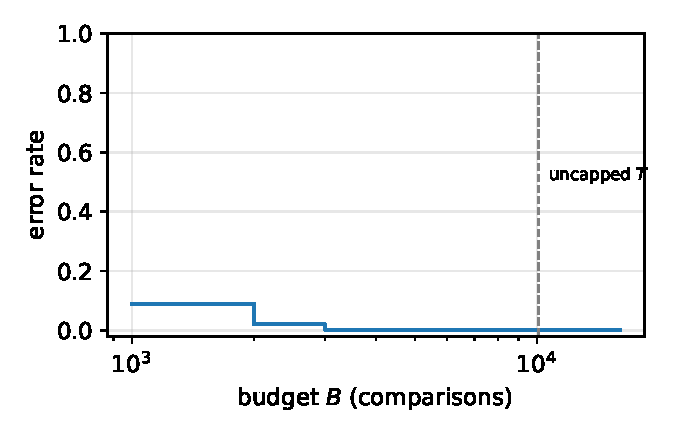
\includegraphics[width=0.6\textwidth]{figures/fig_e4.pdf}
\caption{E4: error rate of Algorithm~\ref{alg:gwe} against the comparison budget ($n=20$, complete graph, $\Delta=0.5$, $k=3$).}
\label{fig:e4}
\end{figure}

\subsection{E5: the uniform-sampling majority-vote baseline}

Table~\ref{tab:e5} compares the standard baseline (sample uniform random edges for a fixed budget, rank by win rate) against Algorithm~\ref{alg:gwe} at $n=20$, $\Delta=0.5$.

\begin{table}[t]
\centering
\caption{E5: majority-vote baseline vs.\ Algorithm~\ref{alg:gwe} ($n=20$, $\Delta=0.5$, $k=3$, 100 repetitions per point).}
\label{tab:e5}
\begin{tabular}{lrrr}
\toprule
graph & baseline behavior & ours: $T$ (mean) & ours: success \\
\midrule
complete & reaches error 0.01 at budget 4000; error $\le 0.05$ from budget 4000 & 10153 & 1.00 \\
cycle & error $\ge 0.90$ at every budget tested (up to 128000) & 13039 & 1.00 \\
\bottomrule
\end{tabular}
\end{table}

On the complete graph the baseline is \emph{cheaper} than our algorithm: it reaches a $0.05$ error rate at budget 4000, a factor 0.39 below Algorithm~\ref{alg:gwe}'s consumption of 10153.  This is expected --- on $K_n$ the win-rate statistic is a faithful Borda proxy and majority voting is statistically efficient, while our calibrated confidence radii buy worst-case robustness at a constant-factor price.  On the cycle the picture inverts sharply: the baseline's error never drops below 0.90 at any budget up to 128000, because on a sparse graph every interior item compares only against its two neighbors and shares (approximately) the same expected win rate, so its win-rate ranking is essentially arbitrary.  Algorithm~\ref{alg:gwe} succeeds with 13039 comparisons.  Graph-aware estimation, not more sampling, is what the restricted-graph setting demands.

\subsection{What the experiments do and do not show}
\label{sec:exp-discussion}
Four observations are recorded against the paper's own claims.  \textbf{(i) Bounded range matters.}  All experiments use bounded-range instances (Condition~\ref{cond:range}, $B=3$).  When we additionally ran unbounded-range (equispaced) instances on the sparse random graph, the practical algorithm mis-eliminated the strongest item in most seeds: its contrast to the boundary must route through chains of saturated edges, whose uncertainty the clipped plug-in radii understate.  This is exactly the regime the bounded-range condition excludes, and a principled one-sided treatment of saturated edges is the main open algorithmic problem.  \textbf{(ii) The worst-case connectivity law is loose for identification.}  E2b's $T^\star$ is essentially uncorrelated with $m_{\mathrm{edges}}/\lG$ across the benign placements (slope -0.06 against the predicted $1$), while E2c shows the law's bite once the boundary straddles a bottleneck (factor 3.92).  Identification cost is governed by the boundary geometry, not by worst-case connectivity alone.  \textbf{(iii) The measured $\Delta$-exponent is between $-1.0$ and $-1.4$, not $-2$.}  The deficit is attributable to the calibrated radii: the Bernstein linear term and the range clip are $\Delta$-independent by construction but bind relatively harder as $\Delta$ grows, and the doubling schedule quantizes the final round.  The $\Delta^{-2}$ information-theoretic benchmark is a lower-bound rate; since all measured success rates are $1.00$ at every $\Delta$, no instance in our sweep contradicts the theory, but our practical algorithm does not visibly exhibit the $-2$ exponent.  \textbf{(iv) Every error rate is measured.}  All success/error rates above are computed from the recorded per-repetition outcomes in \texttt{results/*.json}; none is extrapolated.

\section{Discussion}
\label{sec:discussion}

\paragraph{Model assumptions.}  The BT model is a parametric idealization; win probabilities in applications need not be transitive, and the Borda/Copeland perspectives \cite{shah2015simple,bengs2023identifying,wu2023borda} address ranking functionals that remain meaningful when $\theta$ does not exist.  Our utilities are static; dynamic (drifting) preferences are out of scope.  The bounded-range condition is standard in the top-$k$ literature \cite{chen2017spectral,yang2026graphmonotone} but is an assumption nonetheless, and our practical confidence radii use it as a clip rather than deriving it from first principles.

\paragraph{What is proved and what is calibrated.}  Theorem~\ref{thm:upper} is proved (by reduction to the entrywise MLE analysis of \cite{yang2026graphmonotone,li2021ellinftybounds}) for the one-shot uniform-per-edge estimator.  Algorithm~\ref{alg:gwe} --- the object actually evaluated --- is a calibrated heuristic: active-set confinement, curvature clipping and a Bernstein linear term in the contrast radii.  On the complete graph, where boundary contrasts have direct edges, this heuristic achieves a $100\%$ empirical success rate at every E1/E3 configuration we tested; on sparse graphs with unbounded-range utilities we observed failures (Section~\ref{sec:exp-discussion}), which is precisely the regime the bounded-range condition excludes.  A rigorous sequential analysis of Algorithm~\ref{alg:gwe} itself remains open.

\paragraph{Adaptivity and the $\lG$ penalty.}  Our lower bound covers edge-balanced algorithms; Remark~\ref{rem:adaptive-gap} explains why the fully adaptive rate needs a packing argument we could not complete, and E2 shows empirically that adaptive concentration reduces but does not eliminate the connectivity penalty on the families tested.  Budget-adaptive stopping (fixed-budget rather than fixed-confidence formulations \cite{goldberger2026optimal}) is a natural next step, as is the semi-random graph model of \cite{yang2024topk} as a middle ground between full access and a fixed graph.

\section{Conclusion}
\label{sec:conclusion}

We formulated top-$k$ identification from noisy pairwise comparisons under a fixed, restricted comparison graph and gave, to the best of our knowledge, its first $\lG$-explicit sample-complexity analysis: a one-shot uniform-per-edge estimator achieves $O(m_{\mathrm{edges}}\log(n/\delta)/(\sigma_{\min}\lG\Delta^2))$ comparisons, edge-balanced algorithms need $\Omega(m_{\mathrm{edges}}\log(1/\delta)/(n\lG\Delta^2))$, and both degenerate correctly to the classical complete-graph rates.  Experiments confirm the $\Delta^{-2}$ law and expose both a strength of adaptive concentration (it softens the connectivity penalty) and a sharp failure of naive baselines on sparse graphs.  The two open fronts are the fully adaptive lower bound (Conjecture~\ref{conj:adaptive}) and a rigorous sequential analysis of the practical algorithm.

\bibliographystyle{plain}
\bibliography{refs}

\end{document}
